% TIETOTEKNIIKAN KANDIDAATINTUTKIELMA
\documentclass[utf8,bachelor]{gradu3}
\usepackage[bookmarksopen,bookmarksnumbered,linktocpage]{hyperref}
\usepackage{graphicx}
\usepackage{subcaption}
\addbibresource{Lahteet.bib}

% META

\begin{document}

\title{Reaaliaikaisesti renderöidyn vektorigrafiikan käyttö videopeleissä}
\translatedtitle{Realtime rendered vector graphics in videogames}

\avainsanat{avain1, avain2, avain3}
\keywords{avainsanat englanniksi}
\tiivistelma{
    Tiivistelmä on tyypillisesti 5-10 riviä pitkä esitys työn pääkohdista (tausta, tavoite, tulokset, johtopäätökset).
}
\abstract{
    Englanninkielinen versio tiivistelmästä.
}

\author{Ville Helppolainen}
\contactinformation{\texttt{vivakank@student.jyu.fi}}
%\supervisor{}

% Otsikko ja metatiedot
\maketitle

% Sisällysluettelo
\mainmatter

% Teksti

\chapter{Johdanto}

Videopelejä pelataan nykyään monilla erikokoisilla ja -resoluutioisilla näytöillä. Esimerkiksi Bethesda Softworksin julkaisema Fallout Shelter -peli on saatavilla älypuhelimille, tietokoneille ja pelikonsoleille \parencite{RefWorks:doc:5bd6d887e4b0a1f99c62e6de}. Käyttäessä perinteistä bittikarttagrafiikkaa kehittäjien täytyy tehdä kompromisseja kohdentaessaan pelejään eri tarkkuuksisille näytöille. Vaihtoehtoja ovat kuvan venyttäminen eri kokoihin, mikä tuottaa epätarkkoja tai pikselöityneitä kuvia, tai monen eri kokoisen kuvan tekeminen, mikä lisää työmäärä ja lopullisen pelin tiedostokokoa. \parencite{RefWorks:doc:5bd8319de4b03ae5c9b276b8}

Vektorigrafiikka on yksi ratkaisu näihin ongelmiin. Se sallii kuvan venyttämisen eri kokoiseksi ilman laadun kärsimistä. Vektorigrafiikkatiedosto, kuten SVG, on usein paljon pienempi kooltaan kuin bittikarttatiedosto, kuten PNG \parencites{RefWorks:doc:5bdc5224e4b05afcfde5b159}{RefWorks:doc:5bdc5292e4b05afcfde5b171}. Kuviosta \ref{vertailu} voi huomata, että jos kuvan haluaa esittää skaalattuna alimman rivin kokoiseksi, vasta 512x512 pikselin versiossa on tarpeeksi resoluutiota, eikä se näytä epäselvältä, toisin kuin sitä pienemmät versiot. 512x512 pikselin version tiedostokoko on kuitenkin yli kaksinkertainen suhteessa alkuperäisen SVG-kuvan tiedostokokoon. Jos kehittäjä haluaa pelin tukevan kaikkia kuviossa mainittuja resoluutioita tulee yhteenlasketuksi tiedostokooksi 612 kilotavua, yhdeksän kertaa alkuperäisen SVG-kuvan tiedostokoko.

SVG-tiedosto tukee myös animointia, ja yhdessä tiedostossa voi olla monta animaatiota \parencite{RefWorks:doc:5bd74719e4b0e42e08f6333b}. Tällä tavalla esimerkiksi pelihahmolle saa samaan tiedostoon toimeton-, juoksu- ja hyppyanimaation. \textcite{RefWorks:doc:5bc4a5cce4b080e02f7eff1b} mukaan vektorigrafiikan renderöinti on perinteisesti ollut hidasta, eikä sitä ole voitu suorittaa tarpeeksi nopeasti jotta se olisi kannattavaa. Nykyiset teknologiat ja laitteistot kuitenkin mahdollistavat vektorikuvien esittämisen huomattavasti aiempaa nopeammin. Vektorikuvia on myös mahdollista esittää 3D-gafiikan seassa. \parencite{RefWorks:doc:5bc4a5cce4b080e02f7eff1b} Kysymykseksi jääkin, miksei reaaliajassa renderöidyn vektorigrafiikan käyttö videopeleissä ole yleistynyt, vaikka teknologia sen sallii. Mitä rajoitteita vektorigrafiikoiden käytössä on? Miten vektorigrafiikoita on käytetty aiemmin videopeleissä, miten niitä käytetään nykyään, ja miten niitä voidaan hyödyntää tulevaisuudessa?

Tässä kandidaatintutkielmassa tutkin vektorigrafiikoiden käyttöä videopeleissä kirjallisuuskatsauksen metodein. Pohdin vektorigrafiikoiden etuja ja haittoja verrattuna bittikarttagrafiikoihin 2D-pelien kontekstissa, mutta myös 3D-objektien teksturointia sivuten. Teen myös katsauksen peleissä käytetyn vektorigrafiikan historiasta, nykytilasta ja mahdollisista tulevaisuuden näkymistä.

\begin{figure}[!b]
	\centering
	
\includegraphics[width=1.0\textwidth]{Ghostscript_Tiger_Comparison.pdf}
    \caption{SVG-kuvan ja erikokoisten PNG-kuvien vertailua. Ylemmällä rivillä on alkuperäinen kuva ja alemmalla suurennos yksityiskohdasta.}\label{vertailu}
\end{figure}

\chapter{Vektorigrafiikka}

\section{Vektorigrafiikat ja niiden käyttö}\label{määrittely}

% - Määrittely
% - Ominaisuudet
% - Käyttökohteet
%     * Fontit ja logot
%     * Datan visualisointi ja pohjapiirustukset
%     * Käyttöliittymät (?)
%     * Pelien assetit
%         ~ Banner Saga
%         ~ Guacamelee
%         ~ Scribblenauts

Vektorigrafiikat ovat tietynlaisia tietokoneella generoituja kuvia. Toisin kuin bittikarttagrafiikat, jotka sisältävät jokaisen pikselin väriarvot, vektorigrafiikat sisältävät tietoa pisteistä ja niiden väliin tulevista suorista viivoista, käyristä viivoista ja muista muodoista \parencites{RefWorks:doc:5bdc5224e4b05afcfde5b159}{RefWorks:doc:5bdc5292e4b05afcfde5b171}. Erilaista tietosisältöä ovat esimerkiksi viivan väri, paksuus, katkonaisuus ja käyttäytyminen kulmissa (terävät, pyöreät tai tylpät kulmat). Viivan sisäpuolen voi täyttää yhtenäisellä värillä, liukuvärillä tai kuviolla, ja sitä voi myös leikata toisella viivalla. \parencite{RefWorks:doc:5bd74719e4b0e42e08f6333b} Koska vektorigrafiikan pisteitä ei ole sidottu pikseleihin vaan omaan koordinaatistoonsa, voidaan sitä skaalata minkä kokoiseksi tahansa ilman että laatu kärsii tai tiedostokoko muuttuu \parencite{RefWorks:doc:5bdc5292e4b05afcfde5b171}.

Käytettyjä vektorigrafiikan tiedostomuotoja ovat esimerkiksi Encapsulated PostScript (EPS), Flash (SWF), Adobe Illustrator (AI) ja Scalable Vector Graphics (SVG) \parencite{RefWorks:doc:5bdc5224e4b05afcfde5b159}. Tässä tutkielmassa keskityn vektorigrafiikan tarkasteluun SVG-tiedostomuodon pohjalta, sillä se on W3C:n standardi vektorigrafiikoille. SVG:n spesifikaatio on myös kattavampi kuin esimerkiksi EPS:n \parencite{RefWorks:doc:5bdc900de4b0afdabde32fb7} ja SWF:n \parencite{RefWorks:doc:5bdc9306e4b069b454d8459e}. SVG-tiedostomuoto tukee edellä mainittujen ominaisuuksien lisäksi muun muassa bittikarttakuvien upottamista, tekstien lisäämistä ja animointia. \parencite{RefWorks:doc:5bd74719e4b0e42e08f6333b}

Vektorigrafiikoilla on useita käyttökohteita. \textcite{RefWorks:doc:5bdc5224e4b05afcfde5b159} esittelee käyttökohteiksi muun muassa logot, tekniset piirustukset ja kaaviokuvat. \textcite{RefWorks:doc:5bdd9b5ae4b0954dddb26329} lisäävät käyttökohteisiin esimerkiksi fontit, kartat, käyttöliittymät ja pelit. Seuraavissa kappaleissa esittelen perusteluita miksi vektorigrafiikat soveltuvat hyvin näihin käyttötarkoituksiin.

Yhdestä vektorikuvasta on helppo luoda erikokoisia versioita \parencite{RefWorks:doc:5bdc5224e4b05afcfde5b159}. Esimerkiksi yritysten logot voivat esiintyä monessa eri koossa pienistä käyntikorteista suuriin tienvarsimainoksiin. On siis tärkeää, että logosta on olemassa useita eri resoluutioisia versioita, tai yksi resoluutioriippumaton versio, vektorikuva. Samasta syystä kuin logojen, teksteissä käytettyjen fonttien tulee olla hyvin skaalautuvia. Nykyisin suurimmassa osassa fontteja kirjaimia esittävät kuvat ovatkin juuri vektorikuvia, mikä sallii tekstin esittämisen eri fonttikoilla \parencite{RefWorks:doc:5bdc5224e4b05afcfde5b159}. Vektorikuvaa on myös helpompi muokata kuin bittikarttakuvaa, sillä sen elementit ovat itsenäisiä objekteja \parencite{RefWorks:doc:5bdc5224e4b05afcfde5b159}. Jos yritys haluaa vaihtaa esimerkiksi värejä, fontteja tai elementtien sijoittelua logossaan, onnistuu se vektorikuvan kanssa helposti.

Vektorigrafiikoilla voidaan esittää laadukkaita interaktiivisia kuvaajia \parencite{RefWorks:doc:5bdc736ae4b05afcfde5d6e4}. Artikkelissaan Lang ja Nolan esittelevät R-ohjelmointikielellä tekemäänsä työkalua, jolla pystyy luomaan datasta erinäköisiä SVG-kuvia. Kuvaan pystyy SVG-tiedoston ominaisuuksien johdosta lisäämään interaktiivisia toiminnallisuuksia. Esimerkiksi elementtejä saa animoitua, kun niitä osoitetaan tai klikataan hiirellä, ja liukusäätimestä voidaan säätää kuvassa esitettävää sisältöä. \parencite{RefWorks:doc:5bdc736ae4b05afcfde5d6e4} Myös Googlen Charts API muodostaa SVG-muotoisia interaktiivisia kaavioita sille syötetystä datasta \parencite{RefWorks:doc:5bde1508e4b0afdabde34e20}.

Tietokoneen käyttöliittymät voivat olla toteutettu vektorigrafiikkana. Microsoftin Windows Presentation Foundationia (WPF) käyttävät ohjelmat ovat vektoripohjaisia. WPF lupaa, että kehittäjän ei tarvitse murehtia päätelaitteen monitorin koosta tai resoluutiosta, sillä se hoitaa skaalaamisen sopivan kokoiseksi. \parencite{RefWorks:doc:5bde3d66e4b0a1f99c63ae5a} Unixin työpöytäympäristö KDE 4:n grafiikat ovat vektorigrafiikoita. Työpöytä ja siihen liittyvät elementit ovat joukkoja SVG-kuvia ja niitä muokkaamalla voidaan säätää värejä ja muotoja. Kaikki ikonit ovat SVG-kuvia, mutta reaaliaikaisen renderöinnin sijasta ikonista pyydetään tietynkokoista versiota, joka rasteroidaan välimuistiin. Tällä tavalla parannetaan suorituskykyä, jota vektorikuvan jatkuva uudelleenrenderöinti heikentäisi. \parencite{RefWorks:doc:5bded7f3e4b09dfad48b846c}

Vektorigrafiikoita käytetään peleissä eri tavoin. \textcite{RefWorks:doc:5bdc818be4b0965708b5a0f0} kertoo artikkelissaan kuinka Guacamelee!-pelin eri vaiheissa käytettiin vektorigrafiikoita. Ensimmäiset pelin luonnokset olivat Flashilla tehtyjä vektorianimaatioita. Myös pelin lopulliset grafiikat tehtiin Flashilla, mikä takasi sulavat animaatiot ja säästi muistia. \parencite{RefWorks:doc:5bdc818be4b0965708b5a0f0} \textcite{RefWorks:doc:5bdc7473e4b05afcfde5d742} tekemässä haastattelussa Brittany Aubert kertoo Scribblenauts Unlimited -pelin grafiikoiden olevan vektorikuvia, jotta objekteja voisi venyttää ilman kuvanlaadun kärsimistä. \textcite{RefWorks:doc:5bd88176e4b0afdabde2b8e2} puolestaan kertoo artikkelissan Banner Saga -pelin animointiprosessista. Animoitavat liikkeet kuvattiin ihmisten näyttelemänä ja rotoskoopattiin Flashilla sarjaksi vektorikuvia. Sen jälkeen Flash-animaatiot rasteroitiin joukoksi bittikarttakuvia. \parencite{RefWorks:doc:5bd88176e4b0afdabde2b8e2}

\section{Vektorigrafiikan ja bittikarttagrafiikan eduista ja haitoista}

% - Muokkaus
% - Animointi
% - Tiedostokoko
% - Level of Detail
% - Renderöinti

Vektorigrafiikasta puhuttaessa tulee väistämättä esiin sen erot bittikarttagrafiikkaan. Usein vektorigrafiikka määritelläänkin juuri sillä, mitenkä se eroaa bittikarttagrafiikasta (ks. luku \ref{määrittely}). Kuten aiemmin on jo ilmennyt, vektorigrafiikan olennaisin ero ja etu bittikarttagrafiikkaan verrattuna on sen resoluutioriippumattomuus. Vektorigrafiikalla on myös monia muita etuja bittikarttagrafiikkaan verrattuna, mutta myös monia haittoja. Tässä luvussa erittelen näitä etuja ja haittoja.

Koska vektorigrafiikka koostuu yksittäisistä elementeistä, käyrien muodostamista muodoista, on sitä helppo muokata \parencite{RefWorks:doc:5bdc5224e4b05afcfde5b159}. Bittigrafiikat ovat taas tyhmiä, ne tietävät vain kuvan mitat ja jokaisen yksittäisen pikselin värin, mutta eivät mitään kuvan esittämistä muodoista \parencite{RefWorks:doc:5bdc5292e4b05afcfde5b171}. Esimerkiksi viivalla rajatun alueen värin muuttaminen bittikarttakuvassa on koettu usean internetkeskustelun perusteella ongelmalliseksi \parencites{RefWorks:doc:5bdf1069e4b0a1f99c63c515}{RefWorks:doc:5bdf10ece4b0273295d72f8a}{RefWorks:doc:5bdf119fe4b0b329c55e47c9}. Vektorikuvan kanssa alueen värin vaihtaminen on kuitenkin helppoa, sillä tarvitsee vain määritellä kyseessä olevan elementin täyttöväri. Elementtien liikuttelu onnistuu vektorikuvassa helposti vaihtamalla pisteiden sijainteja, ja taustalla oleva elementti tulee silloin luonnollisesti näkyviin. Sen sijaan bittikarttakuvassa pitää ensin valita kaikki liikutettavat pikselit, jotka sitten liikkuessaan jättävät aukon kuvaan. \parencite{RefWorks:doc:5bdc5224e4b05afcfde5b159}

Vektorigrafiikan elementtipohjaisuus mahdollistaa sen helpon animoimisen. Elementtien ominaisuuksia kuten sijaintia ja väriä pystyy muuttamaan ajan suhteen ohjelmallisesti, jolloin animoijan ei tarvitse määrittää kuin muutama avainkuva ja tietokone luo niiden väliin jäävät kuvat automaattisesti. Bittikartta-animaatiota tehdessä pitää valita käytettävä kehysnopeus ja piirtää sen mukainen määrä yksittäisiä kuvia. \parencite{RefWorks:doc:5bdc5224e4b05afcfde5b159} Jos bittikartta-animaation kehysnopeuden haluaakin esimerkiksi kaksinkertaistaa, tulee myös työmäärä kaksinkertaiseksi. Sen sijaan vektorianimaatio ei välitä ollenkaan kehysnopeudesta, vain animaation kesto tiedetään ja kehysnopeus määräytyy käytettävän laitteiston perusteella. Tehokas tietokone voi siis piirtää monta sataa kuvaa sekunnissa, mutta pienitehoinen kone piirtää vain muutamia kuvia.

Bittikarttagrafiikan suurin etu onkin juuri suorituskyvyssä. Vektorigrafiikkakuvan renderöinti vaatii monia matemaattisia laskutoimituksia, jotta käyriä kuvaavasta datasta saadaan piirrettyä pikseleistä koostuva kuva. Bittikarttakuvaan onkin tallennettu pikseleistä koostuva kuva jo valmiiksi, joten ylimääräistä laskemista ei tule ollenkaan. \parencite{RefWorks:doc:5bdc5292e4b05afcfde5b171} Uusien nopeampien algoritmien kehittäminen vektorigrafiikan renderöimiseen on mielenkiintoinen tutkimuksen kohde. Esimerkiksi \textcite{RefWorks:doc:5bdf538de4b04939ba18218f} esittelevät algoritmia, joka nopeuttaa vektorikuvasta mielivaltaisesti otetun osan renderöimistä. Bittikarttakuvasta on tehokasta ottaa mielivaltainen osa, sillä kaikkien pikselien väri tiedetään jo valmiiksi. Sen sijaan vektorikuvasta mielivaltaisen osan ottaminen on epätehokasta, koska koko kuvan kaikki käyrät on joka tapauksessa pakko laskea. Nehabin ja Hoppen algoritmi tarjoaa ratkaisun tällaiseen ongelmaan. \parencite{RefWorks:doc:5bdf538de4b04939ba18218f} \textcite{RefWorks:doc:5bc4a5cce4b080e02f7eff1b} tarjoavat tehokkaan tavan hyödyntää näytönohjainta perinteisesti prosessorilla tapahtuvaan vektorigrafiikan renderöimiseen.

Vektorikuvan tiedostokokoon suhde bittikarttakuvan tiedostokokoon riippuu kuvan monimutkaisuudesta ja resoluutiosta. Vektorikuvan tiedostokokoon vaikuttaa kuvan monimutkaisuus: mitä enemmän viivoja sitä suurempi tiedosto. Bittikarttakuvan kokoon vaikuttaa sen resoluutio: mitä suurempi kuva sitä suurempi tiedosto. Käyttökohteissa, joissa kuva on yksinkertainen, on vektorikuvan tiedostokoko pienempi. Jos esitetään monimutkaista kuvaa kuten valokuvaa, on bittikarttakuvan tiedostokoko pienempi. Tiedostokoon puolesta vektorikuva on parempi valinta kuin bittikarttakuva yksinkertaiseen grafiikkaan kuten logoon, mutta monimutkaiseen grafiikkaan jossa on paljon yksityiskohtia bittikarttakuva on soveltuvampi. \parencite{RefWorks:doc:5bdf4af9e4b0f02deeb8a48a}

\chapter{Vektorigrafiikat videopeleissä}

\section{Vektorigrafiikan historia peleissä}

% - Oikeat vektoripelit
% - Another World
% - Flash-selainpelit

Vektorigrafiikoilla on ollut merkittävä osa videopelien historiassa. Ensimmäiset graafiset pelit käyttivät näyttöinään oskilloskooppeja ja satunnaisskannausnäyttöjä (random scan display), laitteita, joilla pystyy pikseleiden sijasta esittämään viivoja, vektoreita. Tällaisia näyttöjä sanotaan vektorinäytöiksi. Vektorinäytöillä oli monia etuja rasterinäyttöihin, kuten elementtien helppo pyörittäminen ja koon muuttaminen. \parencite{RefWorks:doc:5be179afe4b05afcfde72671}

William Higinbothanin 1958 kehittämä Tennis for Two (ks. kuvio \ref{tennis}) on yksi ensimmäisistä graafisista videopeleistä \parencite{RefWorks:doc:5be15b13e4b05b9281959f24}. Tennis for Twossa on vain muutama yksinkertainen elementti, viivat esittävät maata, verkkoa ja tennismailoja ja piste esittää palloa, joten se sopii hyvin oskilloskoopilla pelattavaksi. Steve Russellin kumppaneineen vuosina 1961 ja 1962 kehittämä Spacewar! (ks. kuvio \ref{spacewar}) toimi alun perin Massachusetts Institute of Technologyn (MIT) Digital Equipment Corporationilta (DEC) saadulla PDP-1 -tietokoneella, mutta sen suuren suosion seurauksena sitä levitettiin ympäri yliopistoja ja siitä tehtiin versioita eri tietokoneille, tehden siitä ensimmäisen videopelin joka on levinnyt yhden yliopiston ulkopuolelle \parencites{RefWorks:doc:5be15b13e4b05b9281959f24}{RefWorks:doc:5be9d948e4b0304fd3d1692a}.

\begin{figure} [!b]
    \begin{subfigure}[t]{0.5\textwidth}
        \centering
        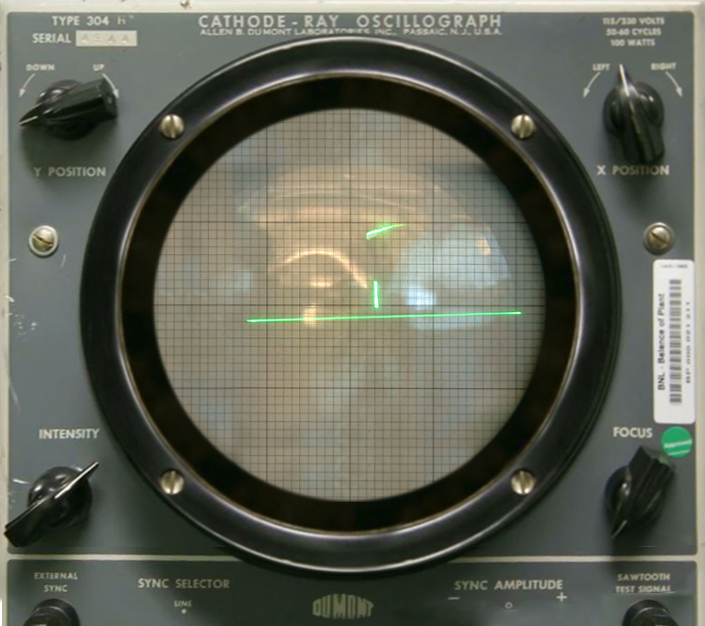
\includegraphics[width=0.8\linewidth]{tennis.jpg}
        \caption{Tennis for Two \parencite{RefWorks:doc:5be168bae4b0273295d7dca5}}\label{tennis}
    \end{subfigure}
    \begin{subfigure}[t]{0.5\textwidth}
        \centering
        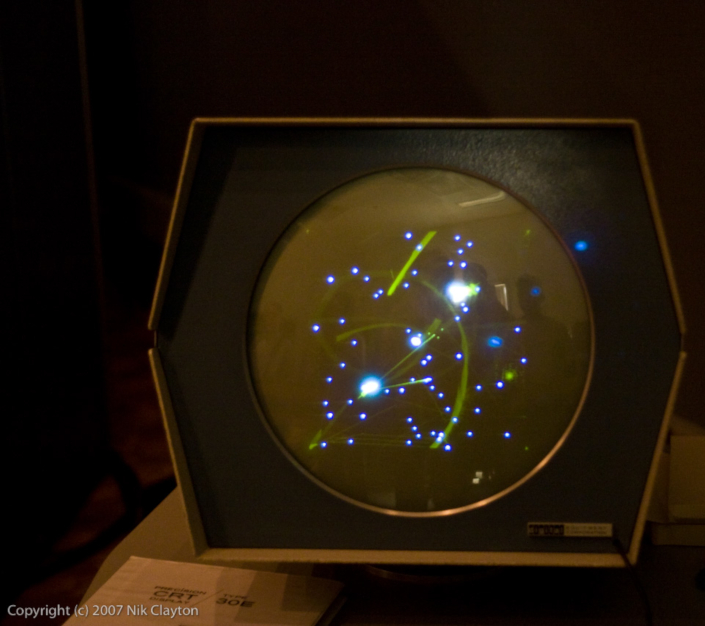
\includegraphics[width=0.8\linewidth]{spacewar.jpg}
        \caption{Spacewar! \parencite{RefWorks:doc:5be162dfe4b0e42e08f77175}}\label{spacewar}
    \end{subfigure}
    \caption{Restauroidut versiot varhaisista videopeleistä.}\label{fig:fig}
\end{figure}

Tennis for Two ja Spacewar! olivat uraa uurtavia videopelejä aikana, jolloin tietokoneet maksoivat satojatuhansia dollareita ja olivat vain vakavaa käyttöä varten. Higinbothan ja Russell ynnä muut kuitenkin osoittivat, että tietokoneista oli paljon muuhunkin, ja turhanpäiväisten ohjelmien ja pelien kehityksestä oli myös käytännöllistä hyötyä. Spacewar! käytti lähes jokaista PDP-1 -tietokoneen käskyä, joten DEC alkoi käyttämään sitä testatessaan ja esitellessään uusien koneidensa toimintaa \parencite{RefWorks:doc:5beac148e4b08968d042364b}. 1970-luvulla videopelejä alettiin tekemään tosissaan ja tuomaan suuren yleisön saataville. 1971 julkaistiin ensimmäiset kolikkopelit Galaxy Game ja Computer Space, jotka molemmat olivat saaneet innoituksensa Spacewar!:sta. 1972 Magnavox julkaisi ensimmäisen kotikonsolin Magnavox Odysseyn. 1977 Apple Computer, Commodore ja Tandy julkaisivat ensimmäiset massatuotetut kotitietokoneet, joista Apple Computerin pelaamiseen keskittynyt Apple II oli kaikkein suosituin. \parencite{RefWorks:doc:5be15b13e4b05b9281959f24}

Ensimmäiset kolikkopelikoneet, pelikonsolit ja kotitietokoneet käyttivät kaikki rasterinäyttöjä, muun muassa sen takia että vektorinäytöt olivat liian kalliita näihin tarkoituksiin. Larry Rosenthal kuitenkin onnistui rakentamaan tarpeeksi halvan vektorinäytön pelihalleihin, ja 1977 julkaistiin ensimmäinen kolikkopeli vektorinäytöllä, Space Wars, joka oli Galaxy Gamen ja Computer Spacen tavoin saanut innoituksensa Spacewar!:sta. Vektorinäytön grafiikat olivat erittäin terävät verrattuna sen aikaisiin pieniresoluutioisiin rasterinäyttöihin, ja ne saivat pelinkehittäjät innostumaan. Syntyi sellaiset klassikkopelit kuin Lunar Lander (1979) ja Asteroids (1979), sekä ensimmäiset 3D pelit Tailgunner (1979) ja Battlezone (1980). Vektorinäyttöjen suosio ei kuitenkaan kestänyt kovin pitkään, kun rasterinäytöistä alkoi tulemaan vuosikymmenten vaihteessa tarkempia ja värikkäämpiä. Vuoden 1983 videopelilaman myötä pelihallit eivät enää tilanneet vektoripelejä, eivätkä vektorinäytöt pysyneet rasterinäyttöjen kehityksen perässä. \parencite{RefWorks:doc:5be15b13e4b05b9281959f24}

Smith Engineeringin kehittämä, 1982 julkaistu Vectrex on ensimmäinen ja ainoa vektorinäytöllä oleva kotikonsoli. Vectrex menestyi melko hyvin, mutta sen menestys ei kestänyt kauaa. Videopelilaman takia sen  valmistus lopetettiin jo 1984. Myöhemmin Vectrex on kuitenkin saanut melko merkittävän aseman retropeliharrastajien keskuudessa, ja se on suosittu alusta omatekoisten pelien tekemiseen. \parencite{RefWorks:doc:5bed604be4b02374b62fe1b5}

\section{Vektorigrafiikan nykytila peleissä}

% - Banner Saga
% - Guacamelee
% - Scribblenauts
% - TF2

\section{Ongelmia vektorigrafiikan käytössä}

% - Ei virallista engine tukea
% - "Rajoittunut" tyyli

\chapter{Pohdintaa vektorigrafiikoiden tulevaisuudesta}

\section{Selainpelit}

% - Selaimessa toimivien sovellusten kasvu
% - Suora tuki SVG:lle ja animaatioille

\section{Vektorigrafiikka 3D-kappaleiden tekstuureissa}

% - Supertekstuurit
% - TF2

\chapter{Yhteenveto}

% - Tarvitaan esimerkki proto

\printbibliography

\end{document}